%
% This file is part of Tangrams-restricted.
%
% Tangrams-restricted is free software: you can redistribute it and/or modify
% it under the terms of the GNU General Public License as published by
% the Free Software Foundation, either version 3 of the License, or
% (at your option) any later version.
%
% This program is distributed in the hope that it will be useful,
% but WITHOUT ANY WARRANTY; without even the implied warranty of
% MERCHANTABILITY or FITNESS FOR A PARTICULAR PURPOSE.  See the
% GNU General Public License for more details.
%
% You should have received a copy of the GNU General Public License
% along with this program.  If not, see <http://www.gnu.org/licenses/>.

\documentclass[USenglish]{article}
% \usepackage[utf8]{inputenx}	% Allow UTF-8 (extended) character encoding
\usepackage[T1]{fontenc}	% Set Type 1 output encoding
\usepackage{csquotes}	% Direct quoting
\usepackage{babel}	% Typesetting for multiple languages (declare language in document class declaration)
\usepackage[backend=bibtex8,sorting=nyt,autolang=hyphen,isbn=false]{biblatex}	% Use BibLaTeX for
% citations
\addbibresource{bib}	% Load a bibliography resource for use by BibLaTeX
\usepackage[USenglish]{datetime2}
\usepackage{graphicx}
\usepackage{dirtree}
\usepackage[breaklinks]{hyperref}	% URL links in document

\graphicspath{{content/}}

% Stylistic macros
\newcommand{\lingform}[1]{\emph{#1}}
\newcommand{\scare}[1]{\textquote{#1}}	% Scare quotes
\newcommand{\term}[1]{{\bfseries #1}}	% Introduction of a new special term
\newcommand{\inlinecode}[1]{\texttt{#1}}	% Inline code; useful for where
% \verb doesn't work 

\newcommand{\corpusname}{KTH Tangrams}

\begin{document}

\title{\corpusname{} Corpus Overview}
\author{Todd Shore \\
KTH Speech, Music and Hearing \\
Stockholm, Sweden \\
{tcshore@kth.se}}	% Remove '\thanks{}' if unneeded
\date{\DTMdate{2018-02-01}}
\maketitle

\tableofcontents

\section{Introduction}

This document describes the corpus \emph{\corpusname{}}, which is a collection of task-oriented dialogues situated in an online board game between two human participants. This collection was done as part of the project \emph{Co-adaptive human-robot interactive systems} (COIN) (\enquote{\"Omsesidig adaption i system f\"or m\"anniska-robotinteraktion}), funded by the Swedish Foundation for Strategic Research from \DTMdate{2016-07-01} to \DTMdate{2021-06-30} (reference number {RIT15-0133}).

Each dialogue in the corpus consists of a pair of participants which alternately assume the roles of \term{instructor}, who has a visual cue of which piece is to be selected on a shared game board, and \term{manipulator}, who must select the piece in question with the help of the instructor's commands (see Figure~\ref{fig:experiment_setup}). These roles are analogous to those of director and matcher in traditional reference communication tasks, with the terms defined by \textcite{Schober&Clark:1989} but the task itself originating from \textcite{Krauss&Weinheimer:1964}. For further information on the experimental setup, see \fullcite{Shore&al:2018}.

\begin{figure}[h]
	\begin{center}
		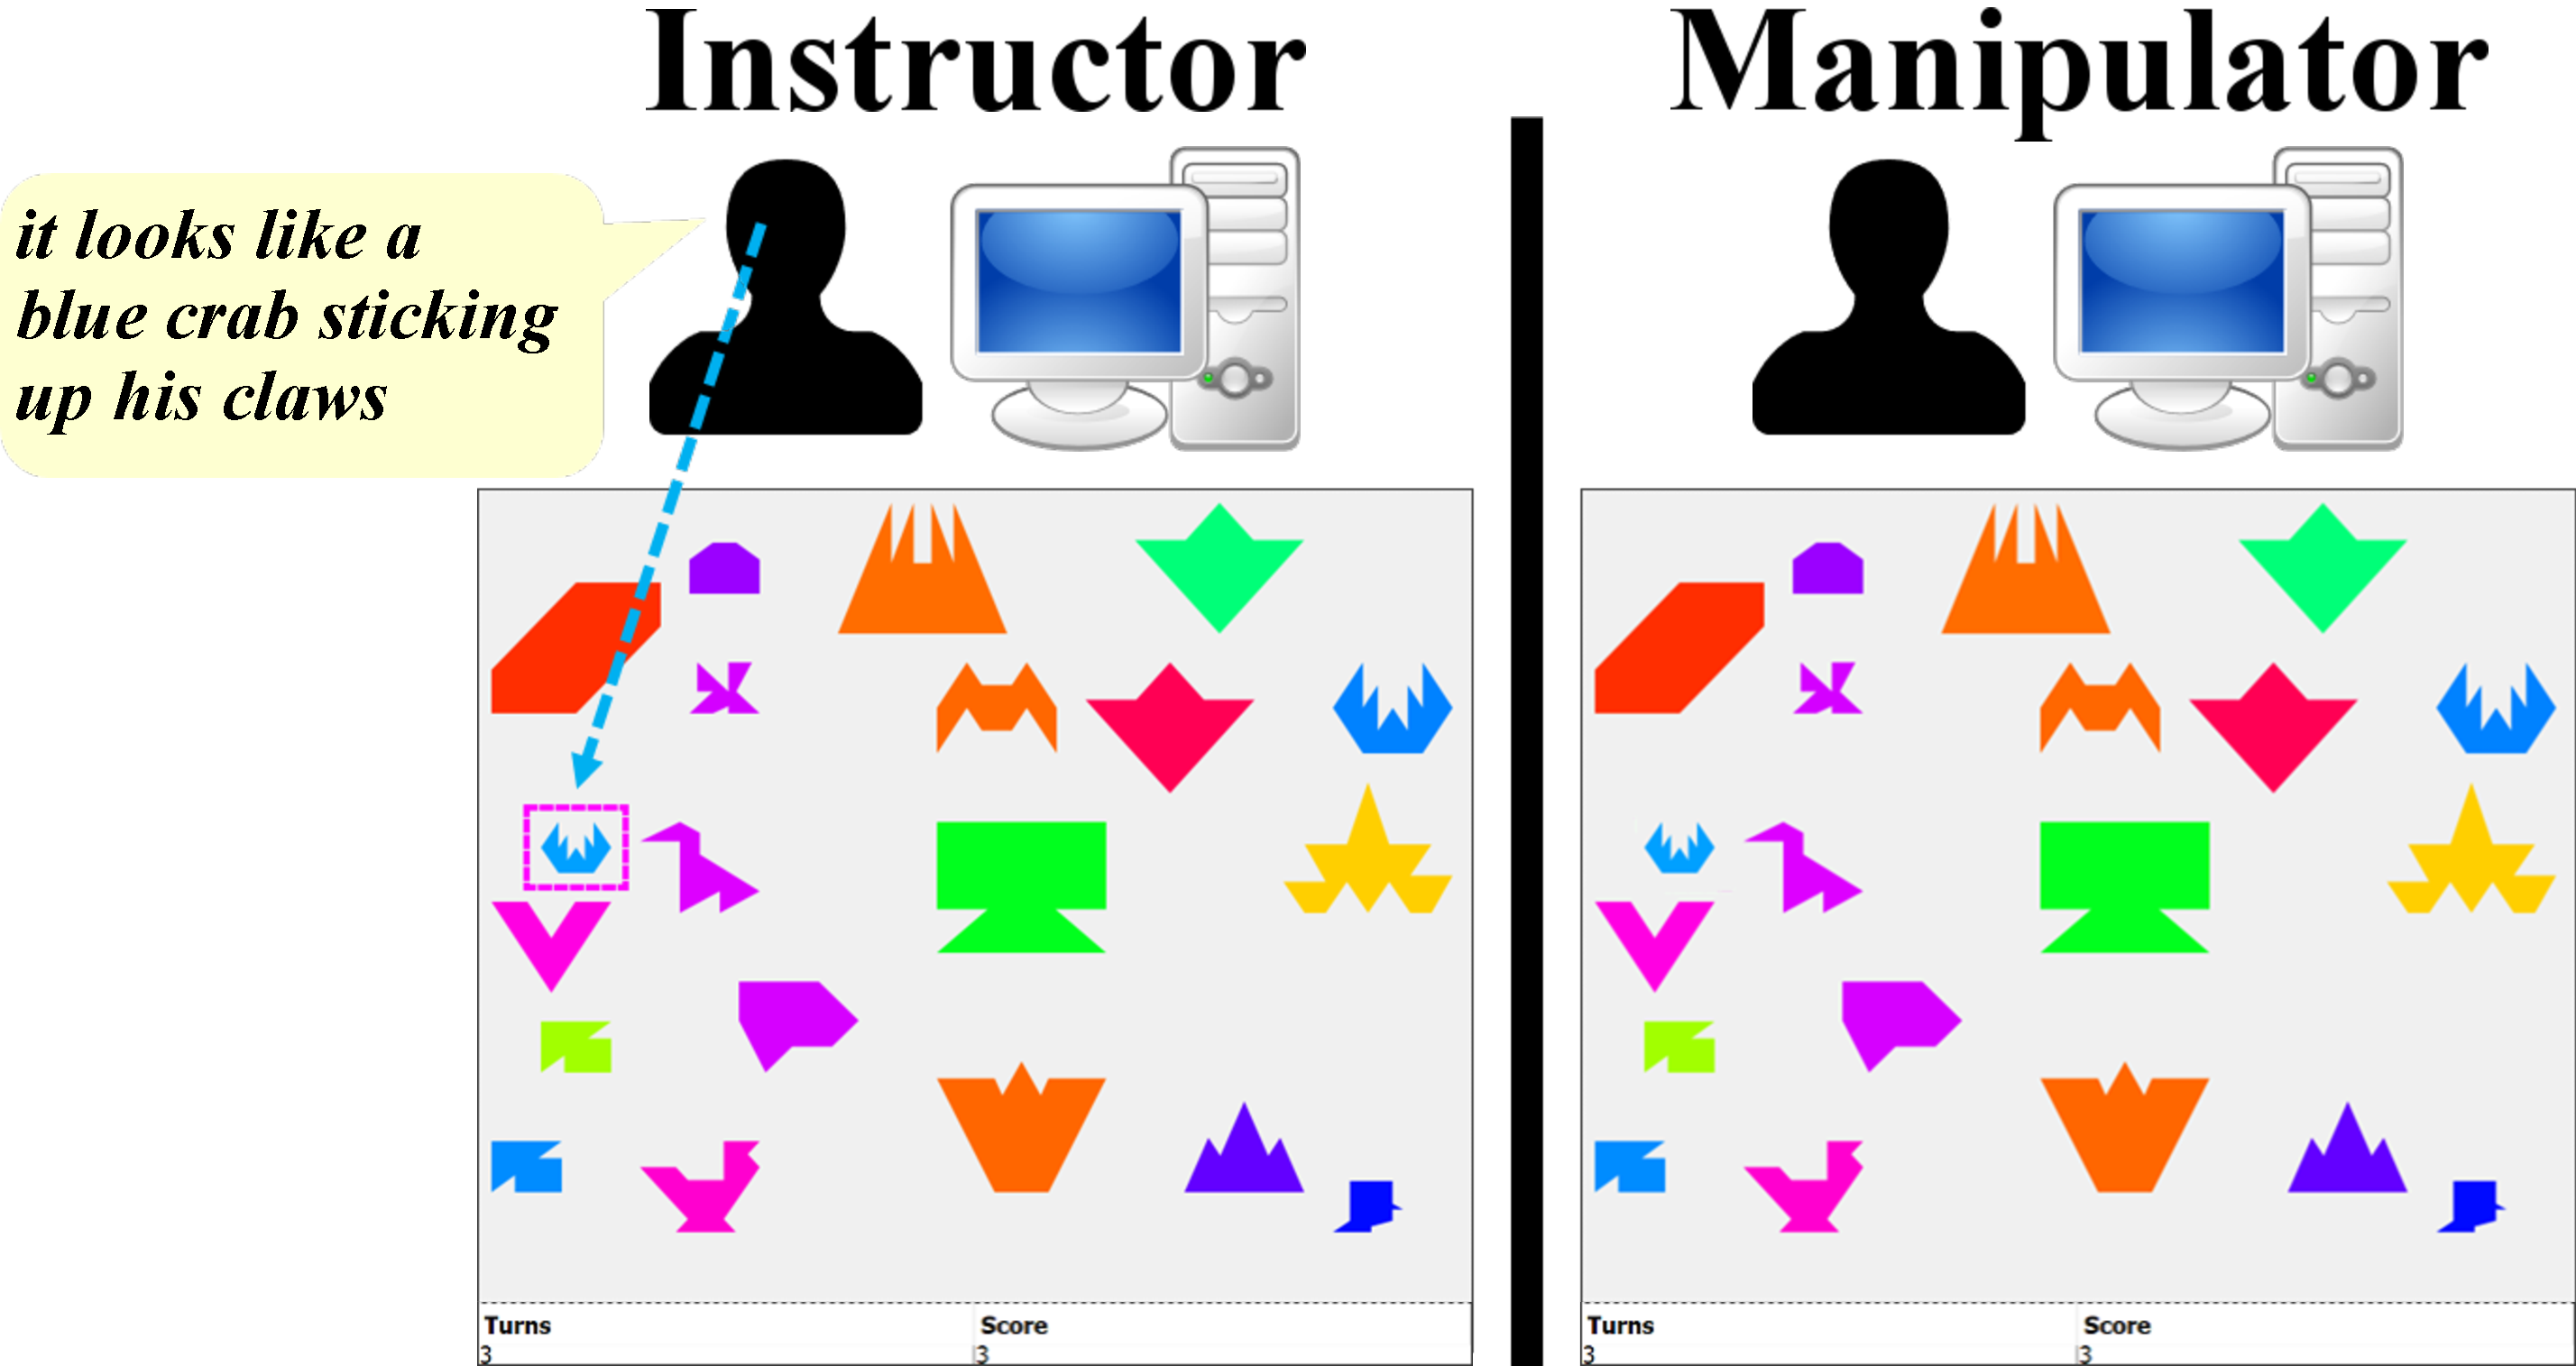
\includegraphics[width=\linewidth]{experiment-setup}
		\caption{The game board as seen by the respective roles.}
		\label{fig:experiment_setup}
	\end{center}
\end{figure}

\section{Data Structure}

The directory \inlinecode{Data} contains the data collected for each dyad, whereby the data for a given dyad is stored in a directory with the dyad ID as the directory name:

%\begin{figure}[h]
\dirtree{%
	.1 <DYAD\_ID>.
	.2 screnshots.
	.3 round-<ROUND\_ID>-<TIMESTAMP>-<PARTICIPANT\_ID>.png.
	.3 selection-entity<ENTITY\_ID>-<TIMESTAMP>-<PARTICIPANT\_ID>.png.
	.2 desc.properties.
	.2 events.tsv.
	.2 events-<PARTICIPANT\_ID>.txt.
	.2 img-info.tsv.
	.2 participant-metadata.tsv.
	.2 session-metadata.tsv.
	.2 system-<PARTICIPANT\_ID>.log.
	.2 utts.tsv.
	.2 utts.xml.	
}
%\end{figure}

\subsection{Session Metadata}

The file \inlinecode{session-metadata.tsv} contains general information about the experimental setup and statistics about the recording session.

\begin{description}
	\item[\inlinecode{END\_SCORE}] The participants' score at the time the recording session ended.
	\item[\inlinecode{ENTITY\_COUNT}] The number of unique entities in the game.
	\item[\inlinecode{EVENT\_COUNT}] The number of events which occurred in the game.
	\item[\inlinecode{EXPERIMENT\_VERSION}] A description of the exact version of experiment software used, comprised of an {ISO-8601} timestamp and Git revision hash.
	\item[\inlinecode{GAME\_DURATION}] The duration of the game in seconds.
	\item[\inlinecode{GAME\_ID}] An integer value used as a seed for randomly-generating values used for entity features\footnote{Random values are generated using a 48-bit seed which is modified using a linear congruential formula \cite[9--25]{Knuth:1981:ACP2} from the Java class library \cite{JavaSE8}}.
	\item[\inlinecode{INITIAL\_INSTRUCTOR\_ID}] The ID of the participant which was first assigned the role of instructor in the game (in the current dataset, always \emph{A}).
	\item[\inlinecode{MOVE\_DELAY}] This is the constant delay in milliseconds between completing a game round and the start of the next round (in addition to latency).
	\item[\inlinecode{ROUND\_COUNT}] The number of game rounds played (but not necessarily completed).
	\item[\inlinecode{START\_TIME}] The time the experiment was started, represented as an {ISO-8601} timestamp
	\item[\inlinecode{ANNOTATOR\_IDS}] A comma-separated list of the unique IDs of each annotator which participated in transcribing the session data.
	\item[\inlinecode{EXPERIMENTER\_ID}] The ID of the person who conducted the experiment; A person's experimenter ID and annotator ID are equivalent.
\end{description}

\subsection{Participant Metadata}

The file \inlinecode{participant-metadata.tsv} contains information about each participant in a dyad, arranged in one column for each participant.

\begin{description}
	\item[\inlinecode{PARTICIPANT\_ID}] The ID of the participant for a given column.
	\item[\inlinecode{INITIAL\_ROLE}] The given participant's initial role, either \emph{MOVE\_SUBMISSION} for instructors or \emph{WAITING\_FOR\_NEXT\_MOVE} for manipulators.
	\item[\inlinecode{SOURCE\_ID}] The ID of the \emph{source} element in the XML-based utterance annotation file \inlinecode{utts.xml} which corresponds to the given participants' audio source: See the \emph{Higgins Annotation Tool} XML schema \cite{HAT}.
	\item[\inlinecode{ACCENT}] A description of the participant's manner of speaking using regional and language terms such as \lingform{Greek}, \lingform{Arabic}, \lingform{Scandinavian (Swedish)}, \lingform{English (General American)}, \lingform{English (Northern England)} or \lingform{South Slavic}. This information is not self-reported but rather assessed by the annotator(s).
	\item[\inlinecode{AGE}] The age of the participant: In the dataset, this is always \lingform{Adult}, i.e.\ above the age of majority, which in Sweden is 18 years of age.
	\item[\inlinecode{DYAD\_PARTNER\_FAMILIARITY}] A description of how familiar the participant is with their partner: \lingform{Strong} indicates close friendship or professional relationship; \lingform{Weak} indicates acquaintanceship such as being classmates or distant colleagues; \lingform{None} indicates complete strangers. This information is not self-reported but rather assessed by the experimenter\slash annotator(s).
	\item[\inlinecode{GENDER}] A description of the participant's manner of speaking using gender-specific terms such as \lingform{masculine} and \lingform{feminine}. This information is not self-assessed but rather assessed by the annotator(s), being evaluated solely on the participant's speech and not on their self-identified gender.
	\item[\inlinecode{SAMPLING\_RATE}] The audio recording sampling rate in hertz.
	\item[\inlinecode{BIT\_DEPTH}] The number of bits of information in each audio recording sample.
	\item[\inlinecode{MICROPHONE}] The microphone used to record the given participant's speech.
	\item[\inlinecode{AUDIO\_CARD}] The audio card used to record the given participant's speech.
	\item[\inlinecode{RECORDING\_LIBRARY}] The software library used for controlling recording of the given participant's speech.
	\item[\inlinecode{SOUND\_SERVER}] The sound server used managing the recording device used.
	\item[\inlinecode{RECORDING\_SOFTWARE}] The software used for writing the recorded audio to disk.
	\item[\inlinecode{COMPUTER}] A description of the computer used by the participant during the experiment.
	\item[\inlinecode{DISPLAY}] The visual display used by the given participant.
	\item[\inlinecode{GRAPHICS\_CARD}] The graphics card used by the given participant.
	\item[\inlinecode{NOTES}] Additional notes about the experiment, the participant themselves, or transcription of the participant's speech.
	\item[\inlinecode{CONSENT\_FORM}] Indicates whether a signed consent form is present for the participant or not.
\end{description}

\subsection{Event Logs}

An event log of all actions in the online game is generated by the client application used by each participant: Each single event in the game is marshalled as a JSON structure using the \emph{IrisTK} framework \autocite{Skantze&AlMoubayed:2012} and are written to the file \inlinecode{events-<PARTICIPANT\_ID>.txt}, whereby participant \emph{A} is the participant which first received the role of instructor, and participant \emph{B} is correspondingly the participant which first received the role of manipulator. In order to facilitate processing without depending on \emph{IrisTK}, a \scare{canonical} event log is written as tab-separated values \autocite{TSV} in \inlinecode{events.tsv}, which is derived from the values in the event log for participant \emph{A}. However, the original participant-specific event logs can still be of use, e.g.\ for calculating round-trip latency from the differences between times of analogous events in the participants' individual logs.

\subsubsection{Records}

Each row in the tabular event log file \inlinecode{events.tsv} represents a record that describes the state of a single entity in the game at a given time.

\begin{description}
	\item[\inlinecode{EVENT}] The ID of the game event the record is attributed to.
	\item[\inlinecode{ROUND}] The ID of the game round during which the event occurred.
	\item[\inlinecode{NAME}] A unique textual identifier of the type of event which occurred: \emph{nextturn.request} occurs at the beginning of a new round and denotes the state of the game at the start of the new round; \emph{selection.request} occurs when a participant selects any piece; \emph{completedturn.request} occurs when the last-selected piece is confirmed as the correct one; \emph{selection.rejection} occurs when the last-selected piece is confirmed as incorrect.
	\item[\inlinecode{SUBMITTER}] The participant who initiated the event.
	\item[\inlinecode{ENTITY}] The ID of the entity the given record describes. 
	\item[\inlinecode{REFERENT}] A Boolean value indicating if the entity the given record describes is the \scare{target} referent, i.e.\ is the entity which must be correctly selected in the given round.
	\item[\inlinecode{SELECTED}] A Boolean value indicating if the entity has been selected by the manipulator or not.
\end{description}

All other values represent physical features of the entity the given record describes.

\subsection{Audio Recordings}

Each experiment session is recorded as a WAV file using linear PCM and two channels --- one channel for each dialogue participant. The two-channel files are then segmented into individual utterances and transcribed into sequences of words (tokens) using the \emph{Higgins Annotation Tool} (HAT) \autocite{HAT}.

When segmenting, annotators were instructed to segment audio into minimals span of uninterrupted language which denote a dialogue act in the scope of the task at hand \autocite[cf.][]{Stolcke&al:2000}. Disfluencies and self-repair delimit segmentation boundaries only if there is a significant period of silence after the potential boundary or if the other participant takes a dialogue turn, leading the participant to respond to the other's speech act \autocite[cf.][]{Schegloff:2000}.

\begin{description}
	\item [Metalanguage] is a set of pre-defined labels, which are always capitalized: \inlinecode{ARTIFACT}, \inlinecode{BREATH}, \inlinecode{CLICK}, \inlinecode{COUGH}, \inlinecode{GASP},	\inlinecode{GROAN}, \inlinecode{GRUNT}, \inlinecode{LAUGHTER}, \inlinecode{MOAN}, \inlinecode{NOISE}, \inlinecode{PUFF}, \inlinecode{SIGH}, \inlinecode{SNIFF}, \inlinecode{START\_SIGNAL}, \inlinecode{UNKNOWN}
	\item [Disfluencies] are indicated with either a leading or trailing hyphen, such as \lingform{-tains} instead of \lingform{mountains} or \lingform{l-} in \lingform{big block l- top left}.
\end{description}

In addition being written in the original HAT XML format in \inlinecode{utts.xml}, the utterance data is also written as tab-separated values in \inlinecode{utts.tsv}:

\begin{description}
	\item[\inlinecode{ROUND}] The ID of the game round during which the utterance occurred.
	\item[\inlinecode{SPEAKER}] The ID participant who made the utterance.
	\item[\inlinecode{DIALOGUE\_ROLE}] The dialogue role of the speaker in the round during which the utterance occurred, either \lingform{INSTRUCTOR} or \lingform{MANIPULATOR}.
	\item[\inlinecode{START\_TIME}] The time the utterance began in seconds from the start of the game.
	\item[\inlinecode{END\_TIME}] The time the utterance ended in seconds from the start of the game.
	\item[\inlinecode{TOKENS}] The utterance transcription in individual tokens (words).
\end{description}

\subsection{Miscellany}

In addition to data about the state of the game and about participants' use of language during the game, there are a number of miscellaneous data sources.

\begin{description}
	\item[Client application logs] are written by the applications used by the individual participants to \inlinecode{system-<PARTICIPANT\_ID>.log}, which may of use for debugging purposes.
	\item[Image visualization data] is written to \inlinecode{img-info.tsv}, which describes static features used for visualizing each entity in the game for a given dyad. Position features are not included because they are dynamic and change throughout the course of the game.
	\item[Screenshots] are saved at the beginning of each new round \linebreak {(\inlinecode{round-<ROUND\_ID>-<TIMESTAMP>-<PARTICIPANT\_ID>.png})} and also for each selection the manipulator makes \linebreak (\inlinecode{selection-entity<ENTITY\_ID>-<TIMESTAMP>-<PARTICIPANT\_ID>.png}); These are stored  under the directory \inlinecode{screenshots}.
	\item[Data structure] information for each session is encoded in the Java properties file \autocite{JavaProperties} \inlinecode{desc.properties}, which maps participant-specific information in utterance XML files to information in \emph{IrisTK} log files. This approach allows use of these files for processing as an alternative to the tabular data files if desired.
\end{description}

%\pagebreak
\printbibliography	% Uncomment to insert BibLaTeX bibliography

\end{document}